% answers.tex —— 2001 年·春季京蒙皖卷·文科 · 参考答案与详细解析片段
% 由 tools/generate_projects.py 依来源总账自 2001/2001_数学真题_春季京蒙皖文_试题.md + 2001/2001_数学真题_春季京蒙皖文_解析正文.md + 2001/2001_数学真题_春季京蒙皖文_答案要点.md 生成，勿手改（改源 MD 后重跑）


\begin{gktip}
固定源 PDF 为印刷页码 81–82 的两页题面，不附答案。以下解析均依据题面独立复算；第 11 题的图形在 LaTeX 工程中以 TikZ/PGFPlots 矢量源重绘。
\end{gktip}

\gkpart{一、选择题}

\begin{answer}
\gksolhead{1}{}

\textbf{题目}：

集合 $M=\{1,2,3,4,5\}$ 的子集个数是\mbox{（　　）}

（A）$32$　　（B）$31$　　（C）$16$　　（D）$15$

\Needspace{4\baselineskip}
\textbf{解析}

\Needspace{5\baselineskip}
集合中有 $5$ 个元素，每个元素都有“取”与“不取”两种选择，所以子集个数为

\nopagebreak[4]
\[
2^5=32
\]

选 A。

\gkanswer{答案：A。}

\end{answer}
\begin{answer}
\gksolhead{2}{}

\textbf{题目}：

函数 $f(x)=a^x$（$a>0$ 且 $a\ne1$）对于任意的实数 $x\text{、}y$ 都有\mbox{（　　）}

（A）$f(xy)=f(x)f(y)$　　（B）$f(xy)=f(x)+f(y)$

（C）$f(x+y)=f(x)f(y)$　　（D）$f(x+y)=f(x)+f(y)$

\Needspace{4\baselineskip}
\textbf{解析}

\Needspace{5\baselineskip}
指数函数满足

\nopagebreak[4]
\[
a^{x+y}=a^xa^y
\]

因此 $f(x+y)=f(x)f(y)$，选 C。

\gkanswer{答案：C。}

\end{answer}
\begin{answer}
\gksolhead{3}{}

\textbf{题目}：

\Needspace{5\baselineskip}
计算

\nopagebreak[4]
\[
\lim_{n\to\infty}\frac{\binom{2n}{n}}{\binom{2n+2}{n+1}}
\]

（A）$0$　　（B）$2$　　（C）$\dfrac12$　　（D）$\dfrac14$

\Needspace{4\baselineskip}
\textbf{解析}

\Needspace{5\baselineskip}
利用组合数的阶乘表示，

\nopagebreak[4]
\[
\frac{\binom{2n}{n}}{\binom{2n+2}{n+1}}
=\frac{(2n)!}{n!n!}\cdot\frac{(n+1)!(n+1)!}{(2n+2)!}
=\frac{n+1}{2(2n+1)}
\]

\Needspace{5\baselineskip}
所以

\nopagebreak[4]
\[
\lim_{n\to\infty}\frac{\binom{2n}{n}}{\binom{2n+2}{n+1}}=\frac14
\]

选 D。

\gkanswer{答案：D。}

\end{answer}
\begin{answer}
\gksolhead{4}{}

\textbf{题目}：

函数 $y=-\sqrt{1-x}$（$x\le1$）的反函数是\mbox{（　　）}

（A）$y=x^2-1$（$-1\le x\le0$）　　（B）$y=x^2-1$（$0\le x\le1$）

（C）$y=1-x^2$（$x\le0$）　　（D）$y=1-x^2$（$0\le x\le1$）

\Needspace{4\baselineskip}
\textbf{解析}

\Needspace{5\baselineskip}
由 $y=-\sqrt{1-x}$ 得 $y\le0$，且

\nopagebreak[4]
\[
y^2=1-x
\Longleftrightarrow
x=1-y^2
\]

交换自变量与因变量，反函数为 $y=1-x^2$，其定义域为 $x\le0$，选 C。

\gkanswer{答案：C。}

\end{answer}
\begin{answer}
\gksolhead{5}{}

\textbf{题目}：

\Needspace{5\baselineskip}
已知 $F_1\text{、}F_2$ 是椭圆

\nopagebreak[4]
\[
\frac{x^2}{16}+\frac{y^2}{9}=1
\]

的两个焦点，过点 $F_2$ 的直线交椭圆于点 $A\text{、}B$，若 $|AB|=5$，则 $|AF_1|+|BF_1|=$\mbox{（　　）}

（A）$11$　　（B）$10$　　（C）$9$　　（D）$16$

\Needspace{4\baselineskip}
\textbf{解析}

\Needspace{5\baselineskip}
椭圆上任意一点到两个焦点的距离之和等于长轴长

\nopagebreak[4]
\[
2a=2\times4=8
\]

\Needspace{5\baselineskip}
因此

\nopagebreak[4]
\[
|AF_1|+|BF_1|=(|AF_1|+|AF_2|)+(|BF_1|+|BF_2|)=8+8=16
\]

选 D。

\gkanswer{答案：D。}

\end{answer}
\begin{answer}
\gksolhead{6}{}

\textbf{题目}：

设动点 $P$ 在直线 $x=1$ 上，$O$ 为坐标原点。以 $OP$ 为直角边、点 $O$ 为直角顶点作等腰直角三角形 $OPQ$，则动点 $Q$ 的轨迹是\mbox{（　　）}

（A）圆　　（B）两条平行直线　　（C）抛物线　　（D）双曲线

\Needspace{4\baselineskip}
\textbf{解析}

\Needspace{5\baselineskip}
设 $P=(1,t)$。将向量 $\overrightarrow{OP}$ 旋转 $90^\circ$，等腰直角三角形的另一个顶点有两种可能：

\nopagebreak[4]
\[
Q=(-t,1)\quad\text{\text{或}}\quad Q=(t,-1)
\]

所以 $Q$ 的轨迹为两条平行直线 $y=1$ 和 $y=-1$，选 B。

\gkanswer{答案：B。}

\end{answer}
\begin{answer}
\gksolhead{7}{}

\textbf{题目}：

已知 $f(x^6)=\log_2x$，那么 $f(8)$ 等于\mbox{（　　）}

（A）$\dfrac43$　　（B）$8$　　（C）$18$　　（D）$\dfrac12$

\Needspace{4\baselineskip}
\textbf{解析}

\Needspace{5\baselineskip}
取 $x=\sqrt2$，则 $x^6=8$，从而

\nopagebreak[4]
\[
f(8)=f\left((\sqrt2)^6\right)=\log_2\sqrt2=\frac12
\]

选 D。

\gkanswer{答案：D。}

\end{answer}
\begin{answer}
\gksolhead{8}{}

\textbf{题目}：

\Needspace{5\baselineskip}
若 $A\text{、}B$ 是锐角三角形 $ABC$ 的两个内角，则点

\nopagebreak[4]
\[
P(\cos B-\sin A,\sin B-\cos A)
\]

在\mbox{（　　）}

（A）第一象限　　（B）第二象限　　（C）第三象限　　（D）第四象限

\Needspace{4\baselineskip}
\textbf{解析}

\Needspace{5\baselineskip}
因 $A\text{、}B\text{、}C$ 都是锐角，且 $A+B=\pi-C>\dfrac\pi2$，有

\nopagebreak[4]
\[
\cos B-\sin A
=\cos B-\cos\left(\frac\pi2-A\right)<0
\]

\Needspace{5\baselineskip}
另一方面，

\nopagebreak[4]
\[
\sin B-\cos A
=\cos\left(\frac\pi2-B\right)-\cos A>0
\]

所以 $P$ 在第二象限，选 B。

\gkanswer{答案：B。}

\end{answer}
\begin{answer}
\gksolhead{9}{}

\textbf{题目}：

如果圆锥的侧面展开图是半圆，那么这个圆锥的顶角（圆锥轴截面中两条母线的夹角）是\mbox{（　　）}

（A）$30^\circ$　　（B）$45^\circ$　　（C）$60^\circ$　　（D）$90^\circ$

\Needspace{4\baselineskip}
\textbf{解析}

\Needspace{5\baselineskip}
设圆锥母线长为 $l$，底面半径为 $r$。侧面展开图为半圆，所以弧长关系给出

\nopagebreak[4]
\[
\pi l=2\pi r
\Longrightarrow r=\frac l2
\]

在圆锥轴截面中，顶角的一半记为 $\theta$，则 $\sin\theta=r/l=1/2$，故顶角为 $60^\circ$，选 C。

\gkanswer{答案：C。}

\end{answer}
\begin{answer}
\gksolhead{10}{}

\textbf{题目}：

若实数 $a\text{、}b$ 满足 $a+b=2$，则 $3^a+3^b$ 的最小值是\mbox{（　　）}

（A）$18$　　（B）$6$　　（C）$2\sqrt3$　　（D）$2\sqrt[4]{3}$

\Needspace{4\baselineskip}
\textbf{解析}

\Needspace{5\baselineskip}
由 $a+b=2$ 及均值不等式，

\nopagebreak[4]
\[
3^a+3^b\ge2\sqrt{3^{a+b}}=2\sqrt9=6
\]

等号在 $a=b=1$ 时取得，选 B。

\gkanswer{答案：B。}

\end{answer}
\begin{answer}
\gksolhead{11}{}

\textbf{题目}：

如图是正方体的平面展开图。在这个正方体中：① $BM$ 与 $ED$ 平行；② $CN$ 与 $BE$ 是异面直线；③ $CN$ 与 $BM$ 成 $60^\circ$ 角；④ $DM$ 与 $BN$ 垂直。以上四个命题中，正确命题的序号是\mbox{（　　）}
\nopagebreak[4]
\begin{center}% 2001 年春季京蒙皖卷第 11 题：正方体平面展开图
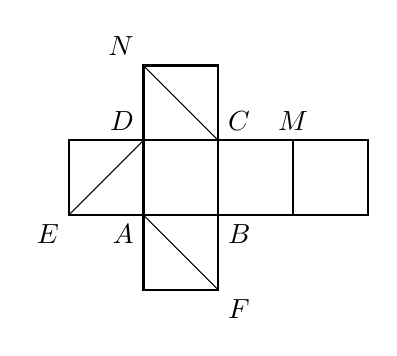
\begin{tikzpicture}[scale=0.95]
  \coordinate (A) at (0,0);
  \coordinate (B) at (1,0);
  \coordinate (C) at (1,1);
  \coordinate (D) at (0,1);
  \coordinate (E) at (-1,0);
  \coordinate (EL) at (-1,1);
  \coordinate (N) at (0,2);
  \coordinate (NT) at (1,2);
  \coordinate (F) at (1,-1);
  \coordinate (FB) at (0,-1);
  \coordinate (M) at (2,1);
  \coordinate (MR) at (2,0);
  \coordinate (RR) at (3,1);
  \coordinate (RRL) at (3,0);

  \draw[thick] (A)--(B)--(C)--(D)--cycle;
  \draw[thick] (E)--(A)--(D)--(EL)--cycle;
  \draw[thick] (D)--(C)--(NT)--(N)--cycle;
  \draw[thick] (A)--(B)--(F)--(FB)--cycle;
  \draw[thick] (C)--(M)--(MR)--(B)--cycle;
  \draw[thick] (M)--(RR)--(RRL)--(MR);
  \draw (E)--(D) (N)--(C) (A)--(F);

  \node[above left] at (N) {$N$};
  \node[above left] at (D) {$D$};
  \node[above right] at (C) {$C$};
  \node[above] at (M) {$M$};
  \node[below left] at (E) {$E$};
  \node[below left] at (A) {$A$};
  \node[below right] at (B) {$B$};
  \node[below right] at (F) {$F$};
\end{tikzpicture}
\end{center}
\nopagebreak[4]
（A）①②③　　（B）②④　　（C）③④　　（D）②③④

\Needspace{4\baselineskip}
\textbf{解析}

\Needspace{5\baselineskip}
按展开图折成立方体，取中央正方形 $ABCD$ 为一个面，设其坐标为

\nopagebreak[4]
\[
A=(0,0,0),\quad B=(1,0,0),\quad C=(1,1,0),\quad D=(0,1,0)
\]

\Needspace{5\baselineskip}
由展开图相邻正方形折叠后可取

\nopagebreak[4]
\[
E=(-1,0,0),\quad N=(0,1,1),\quad M=(1,1,1)
\]

\Needspace{5\baselineskip}
于是

\nopagebreak[4]
\[
\overrightarrow{BM}=(0,1,1),\qquad
\overrightarrow{ED}=(1,1,0)
\]

\Needspace{5\baselineskip}
二者不平行，命题①错误。又

\nopagebreak[4]
\[
\overrightarrow{CN}=(-1,0,1),\qquad
\overrightarrow{BM}=(0,1,1)
\]

\Needspace{5\baselineskip}
所以

\nopagebreak[4]
\[
\frac{\overrightarrow{CN}\cdot\overrightarrow{BM}}
{|\overrightarrow{CN}|\,|\overrightarrow{BM}|}
=\frac12
\]

\Needspace{5\baselineskip}
命题③正确。直线 $BE$ 与 $CN$ 不相交且不平行，命题②正确；此外

\nopagebreak[4]
\[
\overrightarrow{DM}=(1,0,1),\qquad
\overrightarrow{BN}=(-1,1,1)
\]

有 $\overrightarrow{DM}\cdot\overrightarrow{BN}=0$，命题④正确。因此选 D。

\gkanswer{答案：D。}

\end{answer}
\begin{answer}
\gksolhead{12}{}

\textbf{题目}：

\Needspace{5\baselineskip}
根据市场调查结果，预测某种家用商品从年初开始的 $n$ 个月内累积的需求量 $S_n$（万件）近似地满足

\nopagebreak[4]
\[
S_n=\frac n{90}(21n-n^2-5)\qquad(n=1,2,\cdots,12)
\]

按此预测，在本年度内，需求量超过 $1.5$ 万件的月份是\mbox{（　　）}

（A）$5$ 月、$6$ 月　　（B）$6$ 月、$7$ 月　　（C）$7$ 月、$8$ 月　　（D）$8$ 月、$9$ 月

\Needspace{4\baselineskip}
\textbf{解析}

\Needspace{5\baselineskip}
记第 $n$ 个月的需求量为 $T_n=S_n-S_{n-1}$，并令 $S_0=0$。由题设

\nopagebreak[4]
\[
T_n=\frac{-n^2+15n-9}{30}
\]

\Needspace{5\baselineskip}
需求量超过 $1.5$ 万件等价于

\nopagebreak[4]
\[
\frac{-n^2+15n-9}{30}>\frac{45}{30}
\Longleftrightarrow
(n-6)(n-9)<0
\]

在 $1\le n\le12$ 的整数中，只有 $n=7,8$，故选 C。

\gkanswer{答案：C。}

\end{answer}
\gkpart{二、填空题}

\begin{answer}
\gksolhead{13}{}

\textbf{题目}：

已知球内接正方体的表面积为 $S$，那么球体积等于\gkblank{}。

\Needspace{4\baselineskip}
\textbf{解析}

\Needspace{5\baselineskip}
设正方体棱长为 $l$，则 $6l^2=S$。球的直径等于正方体体对角线，所以球半径

\nopagebreak[4]
\[
r=\frac{\sqrt3}{2}l=\sqrt{\frac S8}
\]

\Needspace{5\baselineskip}
球体积为

\nopagebreak[4]
\[
V=\frac43\pi r^3
=\frac43\pi\left(\frac S8\right)^{3/2}
=\frac{\pi\sqrt2}{24}S^{3/2}
\]

\gkanswer{答案：$\dfrac{\pi\sqrt2}{24}S^{3/2}$。}

\end{answer}
\begin{answer}
\gksolhead{14}{}

\textbf{题目}：

椭圆 $x^2+4y^2=4$ 长轴上一个顶点为 $A$，以 $A$ 为直角顶点作一个内接于椭圆的等腰直角三角形，该三角形的面积是\gkblank{}。

\Needspace{4\baselineskip}
\textbf{解析}

\Needspace{5\baselineskip}
取长轴右端点 $A=(2,0)$。设等腰直角三角形的一个直角边向量为 $(u,v)$，另一个取其逆时针旋转 $90^\circ$ 后的向量 $(-v,u)$。两端点在椭圆 $x^2+4y^2=4$ 上，故

\nopagebreak[4]
\[
u+\frac{u^2}{4}+v^2=0,\qquad
-v+\frac{v^2}{4}+u^2=0
\]

\Needspace{5\baselineskip}
令 $s=-u>0$，由两式得

\nopagebreak[4]
\[
s=\frac{s^2}{4}+v^2,\qquad
v=\frac{v^2}{4}+s^2
\]

\Needspace{5\baselineskip}
相减后得到 $(s-v)\left(1+\dfrac34(s+v)\right)=0$，所以 $s=v$，再代回得 $s=4/5$。两直角边长度平方均为

\nopagebreak[4]
\[
s^2+v^2=\frac{32}{25}
\]

\Needspace{5\baselineskip}
三角形面积为

\nopagebreak[4]
\[
\frac12\left(\frac{32}{25}\right)=\frac{16}{25}
\]

\gkanswer{答案：$\dfrac{16}{25}$。}

\end{answer}
\begin{answer}
\gksolhead{15}{}

\textbf{题目}：

\Needspace{5\baselineskip}
已知

\nopagebreak[4]
\[
\sin^2\alpha+\sin^2\beta+\sin^2\gamma=1
\]

（$\alpha\text{、}\beta\text{、}\gamma$ 均为锐角），那么 $\cos\alpha\cos\beta\cos\gamma$ 的最大值等于\gkblank{}。

\Needspace{4\baselineskip}
\textbf{解析}

\Needspace{5\baselineskip}
令 $x=\sin^2\alpha$、$y=\sin^2\beta$、$z=\sin^2\gamma$，则 $x+y+z=1$，且

\nopagebreak[4]
\[
(\cos\alpha\cos\beta\cos\gamma)^2=(1-x)(1-y)(1-z)
\]

\Needspace{5\baselineskip}
由于

\nopagebreak[4]
\[
(1-x)+(1-y)+(1-z)=2
\]

\Needspace{5\baselineskip}
由均值不等式，

\nopagebreak[4]
\[
(1-x)(1-y)(1-z)\le\left(\frac23\right)^3=\frac8{27}
\]

\Needspace{5\baselineskip}
等号在 $x=y=z=1/3$ 时取得。因此最大值为

\nopagebreak[4]
\[
\sqrt{\frac8{27}}=\frac{2\sqrt6}{9}
\]

\gkanswer{答案：$\dfrac{2\sqrt6}{9}$。}

\end{answer}
\begin{answer}
\gksolhead{16}{}

\textbf{题目}：

已知 $m\text{、}n$ 是直线，$\alpha\text{、}\beta\text{、}\gamma$ 是平面，给出下列命题：

①若 $\alpha\perp\beta$，$\alpha\cap\beta=m$，$n\perp m$，则 $n\perp\alpha$ 或 $n\perp\beta$；

②若 $\alpha\parallel\beta$，$\alpha\cap\gamma=m$，$\beta\cap\gamma=n$，则 $m\parallel n$；

③若 $m$ 不垂直于 $\alpha$，则 $m$ 不可能垂直于 $\alpha$ 内的无数条直线；

④若 $\alpha\cap\beta=m$，$n\parallel m$，且 $n\not\subset\alpha$，$n\not\subset\beta$，则 $n\parallel\alpha$ 且 $n\parallel\beta$。

其中正确的命题的序号是\gkblank{}。（注：把你认为正确的命题的序号都填上）

\Needspace{4\baselineskip}
\textbf{解析}

命题①不成立：在两个互相垂直的平面中，取一条既不垂直于其中任一平面、又垂直于交线的直线即可反例。

命题②成立：平行平面被同一平面所截，所得交线互相平行。

命题③不成立：若直线 $m$ 在平面 $\alpha$ 内，则 $m$ 不垂直于 $\alpha$，但平面 $\alpha$ 内有无数条与 $m$ 垂直的直线。

命题④成立：$n$ 平行于交线 $m$，而 $m$ 同时在 $\alpha\text{、}\beta$ 内；又 $n$ 不在这两个平面内，所以 $n$ 分别平行于 $\alpha\text{、}\beta$。故正确命题为②④。

\gkanswer{答案：②④。}

\end{answer}
\gkpart{三、解答题}

\begin{answer}
\gksolhead{17}{}

\textbf{题目}：

方程 $2x^2+mx+n=0$ 有实根，且 $2\text{、}m\text{、}n$ 为等差数列的前三项。求该等差数列公差 $d$ 的取值范围。

\Needspace{4\baselineskip}
\textbf{解析}

\Needspace{5\baselineskip}
设等差数列公差为 $d$，则

\nopagebreak[4]
\[
m=2+d,\qquad n=2+2d
\]

\Needspace{5\baselineskip}
方程有实根的充要条件是判别式非负：

\nopagebreak[4]
\[
\Delta=m^2-8n
=(2+d)^2-8(2+2d)
=d^2-12d-12\ge0
\]

\Needspace{5\baselineskip}
解得

\nopagebreak[4]
\[
d\le6-4\sqrt3\quad\text{\text{或}}\quad d\ge6+4\sqrt3
\]

\gkanswer{答案：$d\in\left(-\infty,6-4\sqrt3\right]\cup\left[6+4\sqrt3,+\infty\right)$。}

\end{answer}
\begin{answer}
\gksolhead{18}{}

\textbf{题目}：

\Needspace{5\baselineskip}
设函数

\nopagebreak[4]
\[
f(x)=\frac{x+a}{x+b}\qquad(a>b>0)
\]

求 $f(x)$ 的单调区间，并证明 $f(x)$ 在其单调区间上的单调性。

\Needspace{4\baselineskip}
\textbf{解析}

\Needspace{5\baselineskip}
函数定义域为 $x\ne-b$，且

\nopagebreak[4]
\[
f'(x)=\frac{(x+b)-(x+a)}{(x+b)^2}
=\frac{b-a}{(x+b)^2}<0
\]

所以 $f(x)$ 在 $(-\infty,-b)$ 和 $(-b,+\infty)$ 上均为减函数。

\gkanswer{答案：$f(x)$ 在 $(-\infty,-b)$ 和 $(-b,+\infty)$ 上均为减函数。}

\end{answer}
\begin{answer}
\gksolhead{19}{}

\textbf{题目}：

已知 $z^7=1$（$z\in\mathbb C$ 且 $z\ne1$）。

（1） 证明 $1+z+z^2+z^3+z^4+z^5+z^6=0$；

（2） 设 $z$ 的辐角为 $\alpha$，求 $\cos\alpha+\cos2\alpha+\cos4\alpha$ 的值。

\Needspace{4\baselineskip}
\textbf{解析}

\gksubpart{(1)}

\Needspace{5\baselineskip}
因为 $z\ne1$，由等比数列求和公式，

\nopagebreak[4]
\[
1+z+z^2+\cdots+z^6=\frac{z^7-1}{z-1}=0
\]

\gksubpart{(2)}

\Needspace{5\baselineskip}
令

\nopagebreak[4]
\[
T=z+z^2+z^4
\]

\Needspace{5\baselineskip}
则 $z^7=1$ 且 $z\ne1$，有 $\overline z=z^6$，从而

\nopagebreak[4]
\[
\overline T=z^6+z^5+z^3
\]

\Needspace{5\baselineskip}
又由上面的七次单位根和式，$T+\overline T=-1$。因此

\nopagebreak[4]
\[
\cos\alpha+\cos2\alpha+\cos4\alpha
=\operatorname{Re}(T)
=\frac{T+\overline T}{2}
=-\frac12
\]

\gkanswer{答案（1）：$1+z+z^2+z^3+z^4+z^5+z^6=0$。}

\gkanswer{答案（2）：$-\dfrac12$。}

\end{answer}
\begin{answer}
\gksolhead{20}{}

\textbf{题目}：

\Needspace{5\baselineskip}
在 $1$ 与 $2$ 之间插入 $n$ 个正数 $a_1,a_2,\cdots,a_n$，使这 $n+2$ 个数成等比数列；又在 $1$ 与 $2$ 之间插入 $n$ 个正数 $b_1,b_2,\cdots,b_n$，使这 $n+2$ 个数成等差数列。记

\nopagebreak[4]
\[
A_n=a_1a_2\cdots a_n,\qquad B_n=b_1+b_2+\cdots+b_n
\]

（1） 求数列 $\{A_n\}$ 和 $\{B_n\}$ 的通项；

（2） 当 $n\ge7$ 时，比较 $A_n$ 与 $B_n$ 的大小，并证明你的结论。

\Needspace{4\baselineskip}
\textbf{解析}

\gksubpart{(1)}

\Needspace{5\baselineskip}
设等比数列公比为 $q$。由首项和末项为 $1\text{、}2$，

\nopagebreak[4]
\[
q^{n+1}=2,\qquad q=2^{1/(n+1)}
\]

\Needspace{5\baselineskip}
因此

\nopagebreak[4]
\[
A_n=q^{1+2+\cdots+n}
=q^{n(n+1)/2}
=2^{n/2}
\]

\Needspace{5\baselineskip}
等差数列公差为 $1/(n+1)$，所以

\nopagebreak[4]
\[
B_n=\sum_{i=1}^n\left(1+\frac{i}{n+1}\right)
=\frac{n(1+2)}2
=\frac{3n}{2}
\]

\gksubpart{(2)}

\Needspace{5\baselineskip}
当 $n=7$ 时，

\nopagebreak[4]
\[
A_7=2^{7/2}=8\sqrt2>\frac{21}{2}=B_7
\]

\Needspace{5\baselineskip}
且

\nopagebreak[4]
\[
\frac{A_{n+1}/B_{n+1}}{A_n/B_n}
=\frac{\sqrt2\,n}{n+1}>1\qquad(n\ge3)
\]

故对所有 $n\ge7$，都有 $A_n>B_n$。

\gkanswer{答案（1）：$A_n=2^{n/2}$，$B_n=\dfrac{3n}{2}$。}

\gkanswer{答案（2）：当 $n\ge7$ 时，$A_n>B_n$。}

\end{answer}
\begin{answer}
\gksolhead{21}{}

\textbf{题目}：

某摩托车生产企业，上年度生产摩托车的投入成本为 $1$ 万元/辆，出厂价为 $1.2$ 万元/辆，年销售量为 $1000$ 辆。本年度为适应市场需求，计划提高产品档次，适度增加投入成本。若每辆车投入成本增加的比例为 $x$（$0<x<1$），则出厂价相应提高的比例为 $0.75x$，同时预计年销售量增加的比例为 $0.6x$。已知年利润 $=$（出厂价$-$投入成本）$\times$年销售量。

（1） 写出本年度预计的年利润 $y$ 与投入成本增加的比例 $x$ 的关系式；

（2） 为使本年度的年利润比上年有所增加，问投入成本增加的比例 $x$ 应在什么范围内？

\Needspace{4\baselineskip}
\textbf{解析}

\gksubpart{(1)}

\Needspace{5\baselineskip}
投入成本增加后，每辆车的成本为 $1+x$ 万元，出厂价为

\nopagebreak[4]
\[
1.2(1+0.75x)=1.2+0.9x
\]

\Needspace{5\baselineskip}
年销售量为 $1000(1+0.6x)$ 辆。因此年利润为

\nopagebreak[4]
\[
y=\bigl[(1.2+0.9x)-(1+x)\bigr]1000(1+0.6x)
=1000(0.2-0.1x)(1+0.6x)
=200+20x-60x^2
\]

\gksubpart{(2)}

\Needspace{5\baselineskip}
上年度利润为 $200$ 万元。要使本年度利润增加，

\nopagebreak[4]
\[
y>200
\Longleftrightarrow
20x(1-3x)>0
\]

\Needspace{5\baselineskip}
结合 $0<x<1$，得

\nopagebreak[4]
\[
0<x<\frac13
\]

\gkanswer{答案（1）：$y=200+20x-60x^2$（万元）。}

\gkanswer{答案（2）：$0<x<\dfrac13$。}

\end{answer}
\begin{answer}
\gksolhead{22}{}

\textbf{题目}：

已知抛物线 $y^2=2px$（$p>0$）。过动点 $M(a,0)$ 且斜率为 $1$ 的直线 $l$ 与该抛物线交于不同的两点 $A\text{、}B$。

（1） 若 $|AB|\le2p$，求 $a$ 的取值范围；

（2） 若线段 $AB$ 的垂直平分线交 $AB$ 于点 $Q$，交 $x$ 轴于点 $N$，试求直角三角形 $MNQ$ 的面积。

\Needspace{4\baselineskip}
\textbf{解析}

\gksubpart{(1)}

\Needspace{5\baselineskip}
直线 $l$ 的方程为 $y=x-a$。与抛物线联立，得

\nopagebreak[4]
\[
x^2-2(a+p)x+a^2=0
\]

\Needspace{5\baselineskip}
设交点横坐标为 $x_1\text{、}x_2$，则

\nopagebreak[4]
\[
x_1+x_2=2(a+p),\qquad x_1x_2=a^2
\]

\Needspace{5\baselineskip}
两根不同要求 $p(p+2a)>0$，即

\nopagebreak[4]
\[
a>-\frac p2
\]

\Needspace{5\baselineskip}
又因直线斜率为 $1$，所以

\nopagebreak[4]
\[
|AB|=\sqrt2\,|x_1-x_2|
=2\sqrt{2p(p+2a)}
\]

\Needspace{5\baselineskip}
中点 $Q$ 的坐标为

\nopagebreak[4]
\[
Q=(a+p,p)
\]

\gksubpart{(2)}

而 $M=(a,0)$，所以 $|QM|=\sqrt2p$。线段 $AB$ 的垂直平分线斜率为 $-1$，与 $x$ 轴交于 $N=(a+2p,0)$，故 $|QN|=\sqrt2p$，且三角形 $MNQ$ 在 $Q$ 处为直角。

\Needspace{5\baselineskip}
因此

\nopagebreak[4]
\[
S_{\triangle MNQ}
=\frac12|QM|\,|QN|
=\frac12(\sqrt2p)^2
=p^2
\]

\gkanswer{答案（1）：$-\dfrac p2<a\le-\dfrac p4$。}

\gkanswer{答案（2）：直角三角形 $MNQ$ 的面积为 $p^2$。}

\end{answer}